%% bare_conf.tex
%% V1.3
%% 2007/01/11
%% by Michael Shell
%% See:
%% http://www.michaelshell.org/
%% for current contact information.
%%
%% This is a skeleton file demonstrating the use of IEEEtran.cls
%% (requires IEEEtran.cls version 1.7 or later) with an IEEE conference paper.
%%
%% Support sites:
%% http://www.michaelshell.org/tex/ieeetran/
%% http://www.ctan.org/tex-archive/macros/latex/contrib/IEEEtran/
%% and
%% http://www.ieee.org/
%%
%%*************************************************************************
%% Legal Notice:
%% This code is offered as-is without any warranty either expressed or
%% implied; without even the implied warranty of MERCHANTABILITY or
%% FITNESS FOR A PARTICULAR PURPOSE!
%% User assumes all risk.
%% In no event shall IEEE or any contributor to this code be liable for
%% any damages or losses, including, but not limited to, incidental,
%% consequential, or any other damages, resulting from the use or misuse
%% of any information contained here.
%%
%% All comments are the opinions of their respective authors and are not
%% necessarily endorsed by the IEEE.
%%
%% This work is distributed under the LaTeX Project Public License (LPPL)
%% ( http://www.latex-project.org/ ) version 1.3, and may be freely used,
%% distributed and modified. A copy of the LPPL, version 1.3, is included
%% in the base LaTeX documentation of all distributions of LaTeX released
%% 2003/12/01 or later.
%% Retain all contribution notices and credits.
%% ** Modified files should be clearly indicated as such, including  **
%% ** renaming them and changing author support contact information. **
%%
%% File list of work: IEEEtran.cls, IEEEtran_HOWTO.pdf, bare_adv.tex,
%%                    bare_conf.tex, bare_jrnl.tex, bare_jrnl_compsoc.tex
%%*************************************************************************

% *** Authors should verify (and, if needed, correct) their LaTeX system  ***
% *** with the testflow diagnostic prior to trusting their LaTeX platform ***
% *** with production work. IEEE's font choices can trigger bugs that do  ***
% *** not appear when using other class files.                            ***
% The testflow support page is at:
% http://www.michaelshell.org/tex/testflow/



% Note that the a4paper option is mainly intended so that authors in
% countries using A4 can easily print to A4 and see how their papers will
% look in print - the typesetting of the document will not typically be
% affected with changes in paper size (but the bottom and side margins will).
% Use the testflow package mentioned above to verify correct handling of
% both paper sizes by the user's LaTeX system.
%
% Also note that the "draftcls" or "draftclsnofoot", not "draft", option
% should be used if it is desired that the figures are to be displayed in
% draft mode.
%
\documentclass[a4paper, 12pt, conference, compsocconf]{IEEEtran}
% Add the compsocconf option for Computer Society conferences.
%
% If IEEEtran.cls has not been installed into the LaTeX system files,
% manually specify the path to it like:
% \documentclass[conference]{../sty/IEEEtran}



% Some very useful LaTeX packages include:
% (uncomment the ones you want to load)


% *** MISC UTILITY PACKAGES ***
%
%\usepackage{ifpdf}
% Heiko Oberdiek's ifpdf.sty is very useful if you need conditional
% compilation based on whether the output is pdf or dvi.
% usage:
% \ifpdf
%   % pdf code
% \else
%   % dvi code
% \fi
% The latest version of ifpdf.sty can be obtained from:
% http://www.ctan.org/tex-archive/macros/latex/contrib/oberdiek/
% Also, note that IEEEtran.cls V1.7 and later provides a builtin
% \ifCLASSINFOpdf conditional that works the same way.
% When switching from latex to pdflatex and vice-versa, the compiler may
% have to be run twice to clear warning/error messages.






% *** CITATION PACKAGES ***
%
\usepackage{cite}
% cite.sty was written by Donald Arseneau
% V1.6 and later of IEEEtran pre-defines the format of the cite.sty package
% \cite{} output to follow that of IEEE. Loading the cite package will
% result in citation numbers being automatically sorted and properly
% "compressed/ranged". e.g., [1], [9], [2], [7], [5], [6] without using
% cite.sty will become [1], [2], [5]--[7], [9] using cite.sty. cite.sty's
% \cite will automatically add leading space, if needed. Use cite.sty's
% noadjust option (cite.sty V3.8 and later) if you want to turn this off.
% cite.sty is already installed on most LaTeX systems. Be sure and use
% version 4.0 (2003-05-27) and later if using hyperref.sty. cite.sty does
% not currently provide for hyperlinked citations.
% The latest version can be obtained at:
% http://www.ctan.org/tex-archive/macros/latex/contrib/cite/
% The documentation is contained in the cite.sty file itself.




%\usepackage{hyperref}

% *** GRAPHICS RELATED PACKAGES ***
%
\ifCLASSINFOpdf
  % \usepackage[pdftex]{graphicx}
  % declare the path(s) where your graphic files are
  % \graphicspath{{../pdf/}{../jpeg/}}
  % and their extensions so you won't have to specify these with
  % every instance of \includegraphics
  % \DeclareGraphicsExtensions{.pdf,.jpeg,.png}
\else
  % or other class option (dvipsone, dvipdf, if not using dvips). graphicx
  % will default to the driver specified in the system graphics.cfg if no
  % driver is specified.
  % \usepackage[dvips]{graphicx}
  % declare the path(s) where your graphic files are
  % \graphicspath{{../eps/}}
  % and their extensions so you won't have to specify these with
  % every instance of \includegraphics
  % \DeclareGraphicsExtensions{.eps}
\fi
% graphicx was written by David Carlisle and Sebastian Rahtz. It is
% required if you want graphics, photos, etc. graphicx.sty is already
% installed on most LaTeX systems. The latest version and documentation can
% be obtained at:
% http://www.ctan.org/tex-archive/macros/latex/required/graphics/
% Another good source of documentation is "Using Imported Graphics in
% LaTeX2e" by Keith Reckdahl which can be found as epslatex.ps or
% epslatex.pdf at: http://www.ctan.org/tex-archive/info/
%
% latex, and pdflatex in dvi mode, support graphics in encapsulated
% postscript (.eps) format. pdflatex in pdf mode supports graphics
% in .pdf, .jpeg, .png and .mps (metapost) formats. Users should ensure
% that all non-photo figures use a vector format (.eps, .pdf, .mps) and
% not a bitmapped formats (.jpeg, .png). IEEE frowns on bitmapped formats
% which can result in "jaggedy"/blurry rendering of lines and letters as
% well as large increases in file sizes.
%
% You can find documentation about the pdfTeX application at:
% http://www.tug.org/applications/pdftex





% *** MATH PACKAGES ***
%
\usepackage[cmex10]{amsmath}
\usepackage{amssymb}
% A popular package from the American Mathematical Society that provides
% many useful and powerful commands for dealing with mathematics. If using
% it, be sure to load this package with the cmex10 option to ensure that
% only type 1 fonts will utilized at all point sizes. Without this option,
% it is possible that some math symbols, particularly those within
% footnotes, will be rendered in bitmap form which will result in a
% document that can not be IEEE Xplore compliant!
%
% Also, note that the amsmath package sets \interdisplaylinepenalty to 10000
% thus preventing page breaks from occurring within multiline equations. Use:
%\interdisplaylinepenalty=2500
% after loading amsmath to restore such page breaks as IEEEtran.cls normally
% does. amsmath.sty is already installed on most LaTeX systems. The latest
% version and documentation can be obtained at:
% http://www.ctan.org/tex-archive/macros/latex/required/amslatex/math/





% *** SPECIALIZED LIST PACKAGES ***
%
%\usepackage{algorithmic}
% algorithmic.sty was written by Peter Williams and Rogerio Brito.
% This package provides an algorithmic environment fo describing algorithms.
% You can use the algorithmic environment in-text or within a figure
% environment to provide for a floating algorithm. Do NOT use the algorithm
% floating environment provided by algorithm.sty (by the same authors) or
% algorithm2e.sty (by Christophe Fiorio) as IEEE does not use dedicated
% algorithm float types and packages that provide these will not provide
% correct IEEE style captions. The latest version and documentation of
% algorithmic.sty can be obtained at:
% http://www.ctan.org/tex-archive/macros/latex/contrib/algorithms/
% There is also a support site at:
% http://algorithms.berlios.de/index.html
% Also of interest may be the (relatively newer and more customizable)
% algorithmicx.sty package by Szasz Janos:
% http://www.ctan.org/tex-archive/macros/latex/contrib/algorithmicx/




% *** ALIGNMENT PACKAGES ***
%
%\usepackage{array}
% Frank Mittelbach's and David Carlisle's array.sty patches and improves
% the standard LaTeX2e array and tabular environments to provide better
% appearance and additional user controls. As the default LaTeX2e table
% generation code is lacking to the point of almost being broken with
% respect to the quality of the end results, all users are strongly
% advised to use an enhanced (at the very least that provided by array.sty)
% set of table tools. array.sty is already installed on most systems. The
% latest version and documentation can be obtained at:
% http://www.ctan.org/tex-archive/macros/latex/required/tools/


%\usepackage{mdwmath}
%\usepackage{mdwtab}
% Also highly recommended is Mark Wooding's extremely powerful MDW tools,
% especially mdwmath.sty and mdwtab.sty which are used to format equations
% and tables, respectively. The MDWtools set is already installed on most
% LaTeX systems. The lastest version and documentation is available at:
% http://www.ctan.org/tex-archive/macros/latex/contrib/mdwtools/


% IEEEtran contains the IEEEeqnarray family of commands that can be used to
% generate multiline equations as well as matrices, tables, etc., of high
% quality.


%\usepackage{eqparbox}
% Also of notable interest is Scott Pakin's eqparbox package for creating
% (automatically sized) equal width boxes - aka "natural width parboxes".
% Available at:
% http://www.ctan.org/tex-archive/macros/latex/contrib/eqparbox/





% *** SUBFIGURE PACKAGES ***
%\usepackage[tight,footnotesize]{subfigure}
% subfigure.sty was written by Steven Douglas Cochran. This package makes it
% easy to put subfigures in your figures. e.g., "Figure 1a and 1b". For IEEE
% work, it is a good idea to load it with the tight package option to reduce
% the amount of white space around the subfigures. subfigure.sty is already
% installed on most LaTeX systems. The latest version and documentation can
% be obtained at:
% http://www.ctan.org/tex-archive/obsolete/macros/latex/contrib/subfigure/
% subfigure.sty has been superceeded by subfig.sty.



%\usepackage[caption=false]{caption}
%\usepackage[font=footnotesize]{subfig}
% subfig.sty, also written by Steven Douglas Cochran, is the modern
% replacement for subfigure.sty. However, subfig.sty requires and
% automatically loads Axel Sommerfeldt's caption.sty which will override
% IEEEtran.cls handling of captions and this will result in nonIEEE style
% figure/table captions. To prevent this problem, be sure and preload
% caption.sty with its "caption=false" package option. This is will preserve
% IEEEtran.cls handing of captions. Version 1.3 (2005/06/28) and later
% (recommended due to many improvements over 1.2) of subfig.sty supports
% the caption=false option directly:
%\usepackage[caption=false,font=footnotesize]{subfig}
%
% The latest version and documentation can be obtained at:
% http://www.ctan.org/tex-archive/macros/latex/contrib/subfig/
% The latest version and documentation of caption.sty can be obtained at:
% http://www.ctan.org/tex-archive/macros/latex/contrib/caption/




% *** FLOAT PACKAGES ***
%
%\usepackage{fixltx2e}
% fixltx2e, the successor to the earlier fix2col.sty, was written by
% Frank Mittelbach and David Carlisle. This package corrects a few problems
% in the LaTeX2e kernel, the most notable of which is that in current
% LaTeX2e releases, the ordering of single and double column floats is not
% guaranteed to be preserved. Thus, an unpatched LaTeX2e can allow a
% single column figure to be placed prior to an earlier double column
% figure. The latest version and documentation can be found at:
% http://www.ctan.org/tex-archive/macros/latex/base/



%\usepackage{stfloats}
% stfloats.sty was written by Sigitas Tolusis. This package gives LaTeX2e
% the ability to do double column floats at the bottom of the page as well
% as the top. (e.g., "\begin{figure*}[!b]" is not normally possible in
% LaTeX2e). It also provides a command:
%\fnbelowfloat
% to enable the placement of footnotes below bottom floats (the standard
% LaTeX2e kernel puts them above bottom floats). This is an invasive package
% which rewrites many portions of the LaTeX2e float routines. It may not work
% with other packages that modify the LaTeX2e float routines. The latest
% version and documentation can be obtained at:
% http://www.ctan.org/tex-archive/macros/latex/contrib/sttools/
% Documentation is contained in the stfloats.sty comments as well as in the
% presfull.pdf file. Do not use the stfloats baselinefloat ability as IEEE
% does not allow \baselineskip to stretch. Authors submitting work to the
% IEEE should note that IEEE rarely uses double column equations and
% that authors should try to avoid such use. Do not be tempted to use the
% cuted.sty or midfloat.sty packages (also by Sigitas Tolusis) as IEEE does
% not format its papers in such ways.





% *** PDF, URL AND HYPERLINK PACKAGES ***
%
%\usepackage{url}
% url.sty was written by Donald Arseneau. It provides better support for
% handling and breaking URLs. url.sty is already installed on most LaTeX
% systems. The latest version can be obtained at:
% http://www.ctan.org/tex-archive/macros/latex/contrib/misc/
% Read the url.sty source comments for usage information. Basically,
% \url{my_url_here}.





% *** Do not adjust lengths that control margins, column widths, etc. ***
% *** Do not use packages that alter fonts (such as pslatex).         ***
% There should be no need to do such things with IEEEtran.cls V1.6 and later.
% (Unless specifically asked to do so by the journal or conference you plan
% to submit to, of course. )

\usepackage{graphicx, graphics}
%\usepackage{array}
%\usepackage{verbatim}
\usepackage[utf8]{inputenc} %% alternativ zu utf8: latin1

%\usepackage{ngerman}
\usepackage{lipsum}

%\usepackage{slashbox}
%\usepackage{rotating}

%\newcolumntype{R}[1]{ %
% >{\begin {turn}{90}\begin {minipage}{#1} %
% \scriptsize \raggedright \hspace {0 pt }}l%
% <{\end{minipage}\end{turn}}%
% }

\newcommand{\todo}[1]{\scriptsize \textbf{TODO:} {#1} \normalsize} % comment
\newcommand{\italic}[1]{\textit{#1}}
\makeatletter
\newcommand{\rmnum}[1]{\romannumeral #1}
\newcommand{\Rmnum}[1]{\expandafter\@slowromancap\romannumeral #1@}
\makeatother

\begin{document}
%
% paper title
% can use linebreaks \\ within to get better formatting as desired
\title{Certificate Authority, its Problems and Alternative Approaches}


% author names and affiliations
% use a multiple column layout for up to two different
% affiliations
\author{\IEEEauthorblockN{Mbombui Nongho Fon-Pah} \\

\IEEEauthorblockA{Uni Duisburg-Essen}}


% conference papers do not typically use \thanks and this command
% is locked out in conference mode. If really needed, such as for
% the acknowledgment of grants, issue a \IEEEoverridecommandlockouts
% after \documentclass

% for over three affiliations, or if they all won't fit within the width
% of the page, use this alternative format:
%
%\author{\IEEEauthorblockN{Michael Shell\IEEEauthorrefmark{1},
%Homer Simpson\IEEEauthorrefmark{2},
%James Kirk\IEEEauthorrefmark{3},
%Montgomery Scott\IEEEauthorrefmark{3} and
%Eldon Tyrell\IEEEauthorrefmark{4}}
%\IEEEauthorblockA{\IEEEauthorrefmark{1}School of Electrical and Computer Engineering\\
%Georgia Institute of Technology,
%Atlanta, Georgia 30332--0250\\ Email: see http://www.michaelshell.org/contact.html}
%\IEEEauthorblockA{\IEEEauthorrefmark{2}Twentieth Century Fox, Springfield, USA\\
%Email: homer@thesimpsons.com}
%\IEEEauthorblockA{\IEEEauthorrefmark{3}Starfleet Academy, San Francisco, California 96678-2391\\
%Telephone: (800) 555--1212, Fax: (888) 555--1212}
%\IEEEauthorblockA{\IEEEauthorrefmark{4}Tyrell Inc., 123 Replicant Street, Los Angeles, California 90210--4321}}




% use for special paper notices
%\IEEEspecialpapernotice{(Invited Paper)}




% make the title area
\maketitle


\begin{abstract}

\lipsum[1]

\end{abstract}

\section{Introduction}

Users of the internet have for over a decade needed a way to securely visit data(mail, websites, servers, etc.). Nonetheless, most frequently accessed data sources cannot for instance actively push their crypto certificates to all of their users (websites like Google would need to exactly know ahead of time who will visit them). Furthermore, pushing a crypto key over the same communication channel that could be a subject to a Man in the Middle (MitM) attack,could cause key learning  vulnerable too. Still internet users require a method to ''securely'' learn crypto certificates for all data sources that they will ever(inlcuding those they may never visit), and acertain if these certifcate holders(named entities) are ''trustworthy'' (that means, a named entity  may still act maliciouly even though it has a valid certificate).\\
\indent Nowaredays, we depend on certain organizations called Certificate Authority(CAs) to do this task  for us. That is, these are organisations the Relyign Parties can trust to confirm both ''\italic{authenticity}'' and ''\italic{trustworthiness}'' of all the named entities' certificates. Each of these CAs  is tied to a certificated of its own. Large software vendors like Apple, Mozilla Foundation, Microsoft, etc often configure  the X.509 certificates for approximately 160 CAs for internet users when their products are installed. These root certificates form the base-line for certificate validation by softwares like web browsers. Here, the reponsibility to choose and update the CA lists is done by the software vendors, and the verification of all data sources that a user may ever visit is done by these root CAs. However the CA Model has some ''weaknesses'' which make it vulnerable to serveral  attacks which are both difficult to detect and/or easy to implement. More details about these liaiblities will be discussed in Section \Rmnum{4} and specific examples in Section \Rmnum{5}\\
\indent The DNS Security Extensions(DNSSEC)[6], [7], [8] has recently become an operationally important technology, and their usage has been growing constantly  for six years now[5]. It has provided the a means for domain owners  to directly manage their security in same distributed database that internet users trust to find their service(DNS). The DNS-Based Authentication of Named Entities(DANE) offers the possibility to use DNSSEC to validate TLS Keys and certificates used by HTTPS and other TLS-based protocols[1]. Furthermore, a couple of commercial products such as Firefox have  add-ons for most browsers while others like Google's Chrome [10] have integrated a native support for the DANE. A remarkable advantage with the DANE approach is that it uses an already existing infrastructure(DNS), which has been used for online transactions and which a vast majority of internet client acting as relying parties(RP) are alread addicted to,(for example it is rare to find a URL that is made up of IP address) attest certificates. Thereby decreasing the system's dependencies on addtional systems  and protocols and consequently reducing the overall attack chances.\\
\indent Perspectives on the other hand tries to prevent these attack by using a collection of ''notary'' servesr that observes named data source's public key through serveral network vantage point and keep records fo a server's key over time . Clients can download these records, when needed and compare them against unauthentuicated keys, there by preventing attacks. Key observations  gathered over the multiple vantage points, makes it difficult for an attacker to compromise all the network paths to destination ,notary data that will allow the client to discover that an attack is eminent(\italic{spial redundancy}) [0]. Futhermore, it enable clients to identify malicious notaries that supply inconsistent data,and there reducing the damage of attack on the notary infrastructure(\italic{data redundancy}).\\
\indent Name Constraints is an extension of X.509 Version 3 certifcate. It defines a name space in which all subsequent certificates in the certification path \textbf{MUST} be located [rfc]. That a top-level domain can only validate certificate of subdomain in its namespace. In case of an attack on a top-level domain(its cerificate is compromised) only certifacates of sub-domains in that namespace will be affected, therey reduicing the attack surface. Details on the above mentioned alternative approaches will be discussed in Section \Rmnum{6}.    


\section{Certificate Authority(CA) Landscape}

Certificate Authority or  Certification Authority(CA), is an organization that is responsible for distributing digital certificates in accordance with a specified Certification Policy. This digital certificate confirms the ownership of a public key by the named subject of the certificate.These CAs make sure that relying parties(RA) can count on  the signatures and assertions made by the private key that matches the public key that is certified.

%In diesem Satz gibt es mehrere Referenzen \cite{Castro02Scribe} \cite{RFC793} %\cite{Wang2006Research}.

\section{Internet X.509 Public Key Infrastructure(PKI) Certificate}
Without certificate authorities and X.509, users would be at risk from having  their TCP connections (SMTP,HTTP, etc) hijacked or compromised. X.509 and certificate authorites are characteristics of public key infrastructure (PKI) schema.\\
\subsection{Overview of PKI Model}
PKI is an infrastructure that provide internet users with the means to securely and privately exchange information through the use of a public and a private key pair obtained and shared through a trusted authority. It also provides digital certificates that matches an individual or organization, a reporsitory that strores and when necessary can revoke the certficates.The component of a public key infrastructure are:\\
End Entity : \indent Users, organizations, or systems who intends to use the private and public technology to securely exchange information.\\
Certificate Authority(CA) : \indent  The oraganization that issues digital certificates binding subject's identity with subjects's public key.\\
Registration Authority(RA) : \indent An optional system to which CA delegate some functions like verifying the subject's identity.\\
Certificate Revocation List(CRL) Issuer: \indent An optional system to which CA delegate the function to publish the Certificate revocation list containing certificates revoked by the CA.\\
Validation Authority(VA) : \indent An optional system to which CA delegate some functions like verifying the digital certificate subject.\\

\begin{figure}[h]
\centering
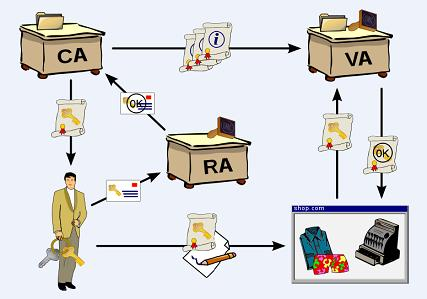
\includegraphics[width=0.7\linewidth]{./figures/PKI_Introduction}
\caption[PKI Workflow]{}
\label{fig:PKI_Introduction}
\end{figure}

\subsection{X.509 Certificate Format}
\subsection{Certificate Validation Process}
\subsection{Subordinate Certificate Authority(SubCA) or Intermidiary CA}



\section{Liabilities: An Assault on One Defeats All}
\input{liabilites}
\section{Prominent Attacks}



\section{Alternative Approaches}
\subsection{DNS-based Authentication of Name Entities(DANE)}
Domain name authentication if a fundamental function for Internet security. In order for applications that communicate over the intertnet to protect their communication from eavesdropping, tampering or forgery, they need to make sure that the entity on the end point of a secure communcation actually reoresents the domain that the user intended to connect to. The Domain Name System Security Extentions (DNSSEC) provides an alternative path for distribution of secure information about domnain names, via Domain Name System(DNS) itself. The DANE working group in the Internet Engineering Task Force(IETF) has developed a new type of DNS record called TLSA record that permits a domain itself to ratify statements about which organisations are empowered to represent or vouch for it. End users' applications can use thes records either to establish a new chain of trust, rooted in the DNS or to increase the existing system of Certificate Authorities.
\subsubsection{TLS Authentication}
The Transport Layer Security(TLS) protocol provides secure client-server connection for many internet applications[2]. In all of these internet applications, the server that the user in the end want to connect to is identified by a DNS domain name[7][8]. An internet user might enter https://example.de into a web browser or send an e.mail to jane@xample.de. So in this case th using the TLS  assures the user that the entity on the other far end of the connection actually represents example.de; that is to certify the server as a true representative of the domain name. It is also to be noted that these comments apply to Datagram Transport Layer Security(DTLS) due to the fact that it provides the same functions as TLS for User Datagram Protocol(UDP) packet flow.
\subsubsection{The TLSA Resource Record(DANE Record)}
The TLSA DNS resource record (RR) is used to match a TLS server certificate or public key with  the domain name where the record is found, thus forming a ''TLSA certificate association''[RFC-6698]. The DANE use cases document[RFC-6698] lays out four main types of statements that permit domain operators to define how clients should judge TLS certificate of their domains. These statements are:
\begin{enumerate}
\item CA Constraints: The client should only accept certifcates published under a specific CA.
\item Service Certificate Constraints: The client should only accept specific certificates for specific services on a host.
\item Trust anchor assertion: The client should use domain-provided trust anchors to validate certificates fo that domain. 
\item Domain-issued Certificate Constraints: The client should only accept certificate issued by the domain name adminstrator itself.
\end{enumerate}
The major difference between the constraints 2. and 4. ist 2. requires that the certificate pass PKIX validation and 4. not.\\
All the above statements can be seen as constraining the scope of trust anchors. The first, second and forth types limits the scope of existing trust anchors; the third type provides the client with a new trus anchor(but still within a limited scope).\\
\indent The DANE TLSA resource record has four major fields:
\begin{itemize}
\item The Certificate Usage Field: This field specifies one of the above mentioned statement types(constraints) as the assoiation that will be used to match the certificate presented in the TLS handshake.
\item The Selector Field: This field specifies which part of the TLS certificate presented by the server with be matched against the association data. That is, the full certificate or its SubjecPublicKeyInfo
\item The Matching Type Field: This field specifies how the certificate association is matched. These types are: Exact match on, SHA-256 hash of and SHA-512 of  selected content[RFC-6234][RFC-6234].
\item The Certificate Association Data Field: This field contains the actual data against which the TLS certificate chain should be matched.
\end{itemize}
\indent The DANE RR is stored under the target domain with a prefix that indicate the port number of the TLS server and the transport protocol on which a TLS-based service is assumed to exist.
\indent TLSA RR Examples: if John runs a secure webservice at john.com and wants to  tell clients to only accept certificates from Jane's CA, he could supply  a TLSA record  under _44_tcp_john.com with following content:
\begin{itemize}
\item Usage: CA constraint
\item Selector: full certificate
\item Matching type: SHA-256
\item Certificate for Association: SHA-256 of Jane's certificate
\end{itemize}
So when client Donald wants to connect to ''https://john.com'', he can find these TLSA RR and appy John's constraint when he validates the server'certificate.
\subsubsection{Comparing DANE to Public CAs}
\subsubsection{Transition Chanllenges}
\subsubsection{Security Considerations}
\subsection{The Perpertive Approach}
\subsection{Name Constraint Approach}
\section{Conclusion}




% trigger a \newpage just before the given reference
% number - used to balance the columns on the last page
% adjust value as needed - may need to be readjusted if
% the document is modified later
%\IEEEtriggeratref{8}
% The "triggered" command can be changed if desired:
%\IEEEtriggercmd{\enlargethispage{-5in}}

% references section

% can use a bibliography generated by BibTeX as a .bbl file
% BibTeX documentation can be easily obtained at:
% http://www.ctan.org/tex-archive/biblio/bibtex/contrib/doc/
% The IEEEtran BibTeX style support page is at:
% http://www.michaelshell.org/tex/ieeetran/bibtex/
%\bibliographystyle{IEEEtran}
% argument is your BibTeX string definitions and bibliography database(s)
%\bibliography{IEEEabrv,../bib/paper}
%
% <OR> manually copy in the resultant .bbl file
% set second argument of \begin to the number of references
% (used to reserve space for the reference number labels box)

\bibliographystyle{IEEEtran}
\bibliography{references}

% that's all folks


\end{document}

